\documentclass{sig-alternate}

\usepackage{url}
\usepackage[table,xcdraw]{xcolor}
\usepackage{eurosym}
\usepackage{amsfonts}
\usepackage{balance}
\usepackage{cite} %this package is awesome - it reorders lists of citations to be in numeric order
\usepackage{pifont}
\usepackage{eqparbox}

% Tables
\usepackage{booktabs}
\usepackage{pbox}
\renewcommand{\arraystretch}{1.2} 
\usepackage{arydshln}
%\renewcommand*\cmidrule{} % No middle lines
%\renewcommand{\arraystretch}{1.5} % Additional spacing with no middle lines
%\renewcommand*\cmidrule{\hdashline[1pt/2pt]}% Dashed middle lines
\renewcommand*\cmidrule{\midrule[0.001em]} % Thin middle lines
%\renewcommand*\cmidrule{\midrule} % Thick middle lines

%Images
%\usepackage[pdftex]{graphicx}
\DeclareGraphicsExtensions{.pdf,.jpg,.png}

\hyphenation{second-ly ap-pen-dix}

\clubpenalty = 10000
\widowpenalty = 10000
\displaywidowpenalty = 10000

\newcommand{\todo}[1]{\textbf{TODO: #1}}
\newcommand{\ms}{LEGO MINDSTORMS EV3}
\newcommand{\mbs}{\textsc{my blocks}}
\newcommand{\mb}{\textsc{my block}}
\newcommand{\horiz}{\hspace{2.1pt}}
\renewcommand{\topfraction}{.9}

\newcommand{\ignore}[1]{}

\begin{document}
%\bstctlcite{IEEEexample:BSTcontrol}
%
% paper title
% can use linebreaks \\ within to get better formatting as desired
\title{A Catalog of OO-inspired End-User Smells, \\and Application to \ms~and Kodu}
%\title{Perspectives on End-User Refactoring: Past, Present, and Future}

\numberofauthors{3}
\author{
% 1st. author
\alignauthor
Felienne Hermans\\
       \affaddr{Delft University of Technology}\\
       \affaddr{Mekelweg 4}\\
       \affaddr{Delft, the Netherlands}\\
       \email{f.f.j.hermans@tudelft.nl}
\alignauthor
Kathryn T. Stolee\\
       \affaddr{Department of Computer Science}\\
       \affaddr{Iowa State University}\\
       \affaddr{Ames, IA, U.S.A.}\\
       \email{kstolee@iastate.edu}
\alignauthor
David Hoepelman\\
       \affaddr{Delft University of Technology}\\
       \affaddr{Mekelweg 4}\\
       \affaddr{Delft, the Netherlands}\\
       \email{D.J.Hoepelman@tudelft.nl}
}
%\author{David Hoepelman, Katryn Stolee, Felienne Hermans}

\maketitle


\begin{abstract}
In the workforce today, millions of people program without degrees or professional training in software development. 
These end-user programmers perform a variety of tasks, from combining web information to building models to support business decisions. Software engineering research into code smells has traditionally focused on professionally used object-oriented programming languages, yet these end-user domains and languages also suffer from code smells. 

In this work, we explore recent research in two distinct end-user domains and languages: spreadsheets in Microsoft Excel and web mashups in Yahoo Pipes. Based on existing OO-smells and their applications to these two end-user domains, we distill a catalog of generic end-user smells. 
We demonstrate the broad applicability of the catalog by mapping the smells to two additional end-user languages not previously targeted by smell detection and refactoring research, both aimed at education: \ms~and Microsoft's Kodu. The results of this application show that  OO inspired smells indeed occur in educational end-user languages and are present in 88\% and 93\% of the EV3 and Kodu programs, respectively. Most commonly we find that programs are plagued with lazy class, duplication, and dead code smells, with the duplication smells being present in nearly 2/3 of programs in each language. We conclude the paper by proposing new end-user smells inspired by the educational languages, moving beyond the OO paradigm. 
\end{abstract}


\section{Introduction}
\todo{make smell names consistent and emph everywhere}
End-user programmers are said to outnumber  professional programmers three times over \cite{Scaf2005}.
These end-user programmers perform a wide variety of tasks within their organizations, ranging from creating new web streams to building and maintaining applications in a spreadsheet. While performing these tasks, end-user programmers, including users of educational languages,  face many of the challenges of professional developers, such as identifying faults, debugging, or understanding code written by someone else~\cite{Ko2011}. 

Similar to code written by professional developers, end-user artifacts may have a long life-span, the average lifespan of a corporate spreadsheet being five years~\cite{Hermans2011}. During this long lifespan, end-user artifacts are modified, often by different people.
These properties make them, like source code artifacts, vulnerable to \emph{smells}. 

The taxonomy of smells outlined in Fowler's text pertained to object-oriented (OO) code, and professional programming languages were the focus for at least the first decade of code smell  and refactoring research~\cite{Mens:2004:SSR:972215.972286}. Recently, however, smells in end-user programming have also reveived attention in research, most notable structural smells in Yahoo Pipes web mashups~\cite{Stolee2011} and Excel spreadsheets \cite{Hermans2012inter}. Experiments in these and other end-user areas have shown that end-user programmers understand smells, and often prefer versions of their code that are non-smelly~\cite{Hermans2012intra, StoleeTSE2013, chambers2013smell}.

% Related is also the work by Chambers and Scaffidi who study performance smells in LabView programming~\cite{chambers2013smell}.

In this paper we combine the two end-user smell approaches and observe that many of the OO smells are applicable in both domains, either they have been already studied, or there is clear opportunity to do so. This led us to the introduction of a generically applicable, OO-inspired end-user smells. To demonstrate the broad applicability of the catalog, we applied it to two new end-user domains aimed at education: \ms~and Microsoft's Kodu. The results of the application show that OO inspired smells in our catalog in fact occur in both end-user languages: 88\% of the EV3 and 93\% of the Kodu programs contained at least one smell. This underlines the power of the code smells concept: they are applicable to visual languages aimed at education, which are quite different from the textual languages aimed at professional developers that the concept was initially designed for. 

In EV3 and Kodu, the smells that we most commonly find are small abstractions (lazy class), duplication, and dead code illustrating commonality across all end-user programming domains. The contributions of this work are as follows:

\begin{itemize}
	\item Synthesis and catalog of object-oriented-inspired code smells in end-user programs
	\item Application of the catalog to two additional end-user domains focused on education: \ms~and Kodu
	\item Identification of future opportunities for domain-specific, non-OO-inspired smell detection in end-user programming domains
\end{itemize}

The rest of this paper is organized as follows. Section~\ref{sec:background} provides background on the two previously studied domains, Excel spreadsheets and Yahoo Pipes mashups. The synthesized catalog of smells is presented in Section~\ref{sec:smells}. We apply the catalog to \ms~and Kodu in Section~\ref{sec:application} by defining each smell in each domain and measuring the presence of smells in corpuses of programs created by children and the community for each language. We explore opportunities for new, non-OO smells in end-user domains in Section~\ref{sec:beyond}, which is followed by related work in Section~\ref{sec:related_work}, threats to validity in Section~\ref{sec:threats} and a conclusion in Section~\ref{sec:conclusions}. 

\section{Background}
\label{sec:background}
In this section we briefly introduce the two end-user languages targeted by prior smell research, before presenting the relevant end-user code smells in Section~\ref{sec:smells}.

\subsection{Excel} Spreadsheets are very commonly used in businesses, from inventory administration to educational applications and from scientific modeling to financial systems.
Winston~\cite{Wins2001} estimates that 90\% of all analysts in industry perform calculations in spreadsheets. 
Microsoft Excel is by far the most used, and therefore most studied, spreadsheet program, but other implementations exists and are similar.

In modern spreadsheet programs, a \textit{cell} can contain a single \textit{formula} which performs a calculation, and a table of cells is bundled in a \textit{worksheet}; an example is shown in Figure~\ref{fig:spreadsheetexample}. 
A \textit{workbook} consist of a collection of worksheets.
Formulas can reference other cells in the same or in different workbooks and worksheets.



\subsection{Yahoo Pipes}
Yahoo Pipes was\footnote{We use the past tense as the Yahoo Pipes environment has been discontinued as of September 30, 2015.} a popular web mashup language and environment with which RSS feed information could be collected and combined from various sources.  Figure~\ref{fig:ypexample} shows an example program as it appeared in the Pipes Editor. The boxes represent modules connected by wires and data flows from the data sources at the top  (e.g., \emph{fetch feed} modules) to the output at the bottom (i.e., \emph{pipe output}). The wires connect the output of a module with either the input or a field of another module. 

Various manipulations of the data are possible along the  way, such as concatenating RSS feeds (e.g., \emph{union} modules), sorting  or filtering based on various criteria, or truncating the list (e.g., \emph{truncate} modules). 
Abstraction was possible with \emph{subpipe} modules, which allowed a programmer to insert a different pipe as a subroutine. These subpipes appeared like a standard module but when clicked, opened the abstracted pipe in an editor. 


\begin{figure}[htb]
\caption{Microsoft Excel 2013 showing a spreadsheet. Columns B and C show the typical mix of data and calculation. The formula of the selected cell B13 is visible right above the spreadsheet.}
\centering
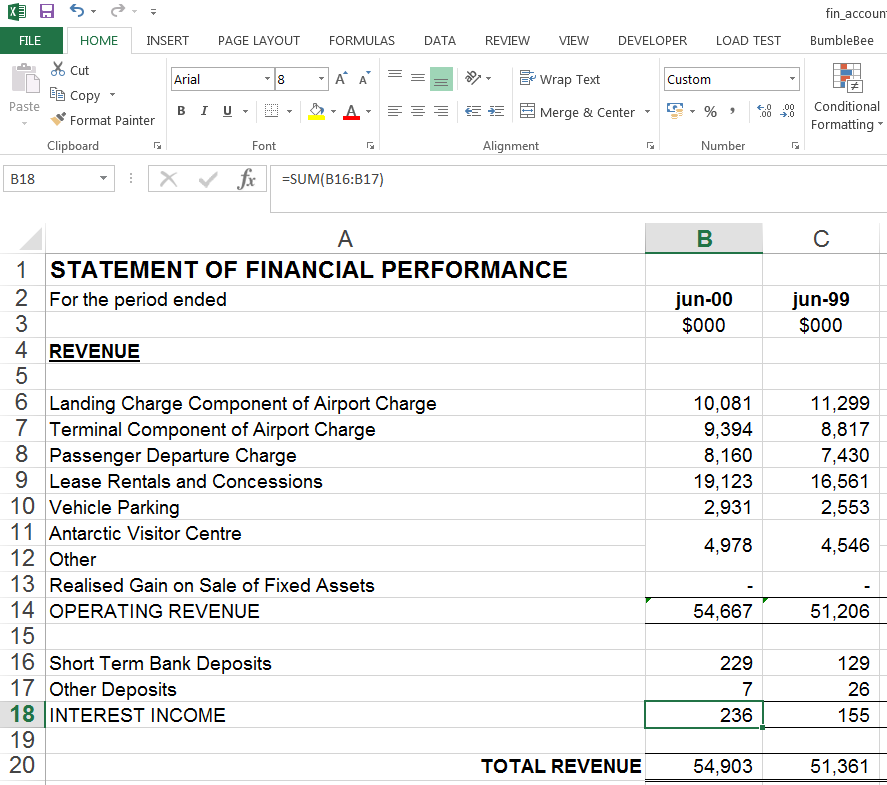
\includegraphics[width=\columnwidth]{img/excel-2}
\label{fig:spreadsheetexample}
%file: fin_accounts from Euses / financial
\end{figure}

\begin{figure}[h!tb]
\caption{Example of a program in Yahoo Pipes. It has five RSS feed data sources, each in a \emph{fetch feed} module, feeding to a \emph{union} module that concatenates the feeds, a \emph{truncate} module that limits the number of items to 15 prior to the final \emph{pipe output}. }
\centering
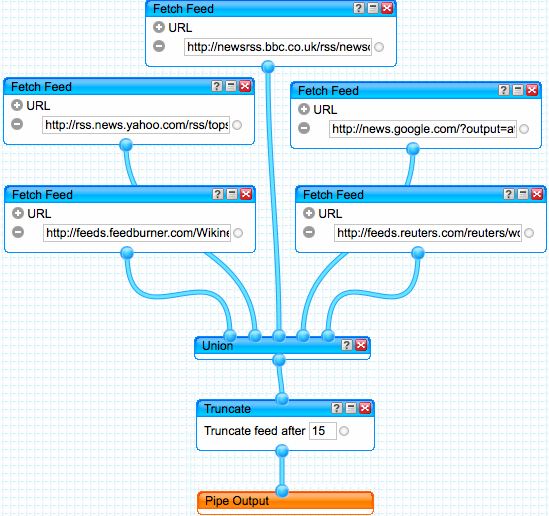
\includegraphics[width=\columnwidth]{img/yp-1}
\label{fig:ypexample}
\end{figure}


\section{Smells in end-user programs}
\label{sec:smells}
Research into end-user language smells has had two approaches, which are not mutually exclusive.
The first approach is to take existing smells for OO programming languages, usually those defined by Fowler~\cite{Fowl1999}, and transform them to be applicable to the end-user environment \cite{Hermans2012inter,Hermans2012intra,Stolee2011,StoleeTSE2013, chambers2013smell}.
The second approach is to define smells tailored to the end-user environment.
This can be done by interviewing experienced end-users to see which smells they perceive \cite{chambers2013smell}, by looking at user reports like forum or newsgroup posts~\cite{badame2012refactoring,chambers2013smell}, or by analyzing publicly available repositories~\cite{Stolee2011,StoleeTSE2013,Hermans2012intra}.


This section provides an overview of different OO-inspired smells that researchers have found to be applicable to end-user artifacts. 
 We catalog the OO smells present in two end-user languages, Excel spreadsheets and Yahoo Pipes mashups, in Table~\ref{table:oosmellslarge}, as identified in prior work~\cite{Stolee2011,StoleeTSE2013,Hermans2012intra, Hermans2012inter}.
 Overall, we often observe similarities in the code smells studied. Specifically, the \emph{duplicate code}, \emph{lazy class}, and \emph{long method} smells  have been studied in both languages. 
Next, we briefly explore some of the studied smells in these two domains. 



\begin{table*}
\caption{Catalog of Code Smells in End-User Programs
\label{table:oosmellslarge}}
\centering
\sffamily
\begin{tabular} {@{}llll@{}}
\toprule
\textbf{OO Smell}
	& \textbf{Excel}
	& \textbf{Yahoo Pipes}
\\ \midrule
Dead Code
	& %~\ding{55}
	& Unnecessary Module \cite{StoleeTSE2013}
\\ \cmidrule
Deprecated Interface
	& %Deprecated Functions *
	& Deprecated Module or Invalid Source \cite{StoleeTSE2013}

\\ \cmidrule
Duplicate Code
	& Duplicated Formulas \cite{Hermans2012intra}
	& Duplicate Modules, Duplicate String or
\\ % Continuation
& 
& Isomorphic Paths \cite{StoleeTSE2013}
\\ \cmidrule
Feature Envy
	& Feature Envy \cite{Hermans2012inter}
	& %Feature Envy *
\\ \cmidrule
Inappropriate Intimacy
	& Inappropriate Intimacy \cite{Hermans2012inter}
	& %Inappropriate Intimacy *
\\ \cmidrule
Lazy class or Middle Man
	& Middle Man \cite{Hermans2012inter}
	& Unnecessary Abstraction \cite{StoleeTSE2013}
\\ \cmidrule
Long Method
	& Multiple Operations \cite{Hermans2012intra}
	& Noisy Module : Duplicate Field \cite{StoleeTSE2013}
\\ \cmidrule
Many Parameters
	& Multiple References \cite{Hermans2012intra}
	& 
\\ \cmidrule
Message Chain
	& Long Calculation Chain \cite{Hermans2012intra}
	& 
\\ \cmidrule
No-op
	& %Redundant Operations *
	& Unnecessary Module \cite{StoleeTSE2013}
\\ \cmidrule
Unused Field
	& %~\ding{55}
	& Noisy Module : Empty Field \cite{StoleeTSE2013}
\\ \bottomrule
%\multicolumn{4}{c}{} \\
%\multicolumn{4}{l}{\ding{55} : Not applicable due to the nature of the paradigm} \\
%\multicolumn{4}{l}{* : Proposed smell, likely future opportunity not supported by prior work}\\
%\multicolumn{4}{l}{$\langle$blank$\rangle$ : Not discussed in this work, possible future opportunity} \\
\end{tabular}
\end{table*}


 \subsection{Excel}
Hermans et al. \cite{Hermans2012inter,Hermans2012intra} analogize a workbook to a program, a worksheet to a class inside that program and a cell to a method and use this to adapt nine of Fowler's smells~\cite{Fowl1999} to the spreadsheet domain.
An example of this is the \emph{long method} smell, which translates to the \emph{multiple operations} smell, since formulas with a large number of operations suffer from similar problems as long methods in terms of understandability and similarly the \emph{many parameters} smell applies to spreadsheet formulas that refer to a large number of other cells or ranges. 

The above two smells occur at the formula level, but smells at the worksheet level occur too. For example, the \emph{feature envy} smell occurs where a given formula mainly uses cells located on a different worksheet, such as: \begin{quote} \begin{small}{\tt =('Required Funds'!B9/'Required Funds'!C9/12) + ('Required Funds'!B10/'Required Funds'!C10/12) + ('Required Funds'!B11/'Required Funds'!C11/12)}, \end{small}\end{quote} which is taken from the clienttemplate.xlsx spreadsheet from the EUSES corpus~\cite{fisher2005euses}. As this formula refers to cells from the {\tt Required Funds} worksheets, it would fit there better. Similarly, two worksheets can have formulas that refer to each other heavily, introducing the \emph{inappropriate intimacy} smells. The \emph{message chain} smell occurs within spreadsheets if long chains of connecting formulas are constructed, hindering understandability as the entire chain has to be traced. In an study on the above mentioned EUSES corpus, 42\% of spreadsheets were found to be smelly~\cite{Hermans2012intra}.

\subsection{Yahoo Pipes}
Stolee and Elbaum~\cite{Stolee2011, StoleeTSE2013} treat a Yahoo Pipes mashup as a class and each module as a method.  Fields in a module are treated as parameters. Using this analogy,  several OO smells were mapped to this language. The most common smell, appearing in nearly one-third of the 8,000 pipes studied, was \emph{duplicate strings}, an instance of Fowler's \emph{duplicate code} smell. 
A similar smell, \emph{duplicate modules}, impacted nearly one-quarter of the pipes studied. 
% Overall, 81\% of the programs studied from the Yahoo Pipes community had at least one smell. 
 
\emph{Dead code} can appear in Yahoo Pipes when a module is not connected to the rest of the pipe. A  \emph{deprecate module} occurs when a program uses a module that has been deprecated in the API. A \emph{lazy class} or \emph{no-op} smell occurs when data flows through an entire pipe or a module, respectively, but is not manipulated. The \emph{unused field} smell occurs when blank fields are left in modules, specifically when those blanks are supposed to contain data sources. Considering the smells in Table~\ref{table:oosmellslarge}, 81\% of over 8,000 programs were found to be smelly~\cite{Stolee2011,StoleeTSE2013}.

\subsection{Summary}
In both the Excel and the Yahoo! Pipes work, OO inspired smells were applied to end-user languages. Some of the smells have been already studied in both domains, while others have not. However, the absence of an entry in Table~\ref{table:oosmellslarge} does not mean the absence of the smell in that language, it simply means such smells have not been studied. While measuring the occurrence of these smells falls outside the scope of the current work, we speculate
that some of these unstudied smells may be applicable. 
For example, \emph{many parameters} is not discussed in previous work on Yahoo Pipes, but could apply when a pipe module receives many field values via wire from other modules. 
Similarly, \emph{no-op} could occur in Excel in a formula like {\tt SUM(A1+A2+A3)}. Here, the {\tt SUM} function does not add anything because it is only sums one value: the result of the addition. 


\begin{figure} [ht]
\caption{The interface of \ms~showing a line following program.}
\centering
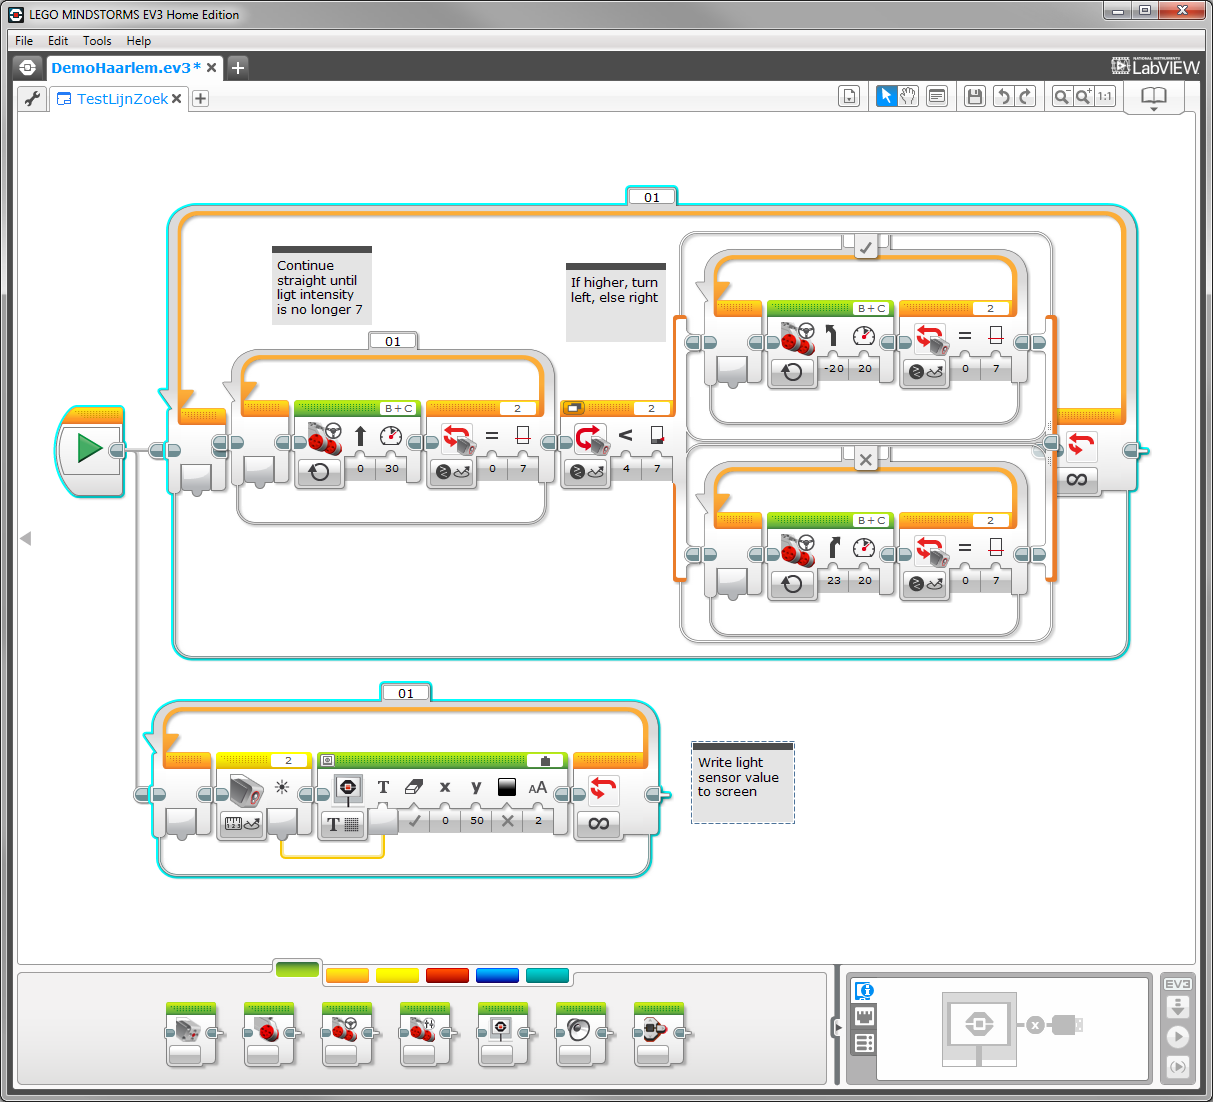
\includegraphics[width=\columnwidth]{img/ms}
\label{fig:ms}
\end{figure}


%\subsubsection{Other Domains}
%End-user programming domains extend beyond spreadsheets and web mashupss. Stolee and Elbaum explore future opportunities for refactoring in educational programming languages~\cite{StoleeTSE2013}. \todo{revisit, this is a bit strange now this paper talks about education too}

%Other end-user programming domains that could benefit from smell analysis and refactoring are mathematical environments like MATLAB, Sage, and Mathematica.

%In particular, the smells related to duplication and poor construction like \emph{long method}, \emph{Many Parameters} and \emph{Dead Code} are prevalent in the four domains studied.
%These smells -- and their respective refactorings -- likely exist in other end-user programming domains, and likely hinder the understandability and maintainability of those programs. Worse even, these smells could lead to errors, and thus these smells are worthy of our attention. 

%\subsection{Future Opportunities in Professional Languages}
%In end-user programming languages, it has been shown that code smells impact the understandability of
%source code~\cite{StoleeTSE2013}. Additionally, being presented with code smells can motivate end-user programmers to improve their code~\cite{chambers2013smell}, and smells in spreadsheets have even been known to reveal actual errors~\cite{Hermans2012intra}. These lessons could extend to professional programming languages. but further study is needed. 
% outside of the end-user programming domains. 
%There has been successful in using automating smell detection, for example, during agile development (e.g.,~\cite{Schumacher:2010:BES:1852786.1852797}). Paired with the end-user evidence, a stronger case can be made to integrate automated smell detection in many domains. 

%\todo{Other data flow languages could benefit from \emph{normalize order of operations} to improve understandability (as it does with YP). }


\section{Application}
\label{sec:application}
In Section~\ref{sec:smells}, we cataloged OO-inspired end-user smells from previous work. In order to demonstrate the applicability of our catalog, we apply it to two new domains: \ms~software (EV3 for short) and  Kodu. 

\subsection{\ms}
\label{sec:lego}
EV3 is the third iteration of the LEGO MINDSTORMS robotics line. It consists of a number of sensors, four motors and an ARM 9 ``intelligent brick''. The robotics kit comes with a control software package, which allows for visual programming of the brick, based on LabView\footnote{\url{http://www.ni.com/labview/}}. The software supports several basic constructs common to programming, including loops and conditionals, but also more advanced features like parallel execution. Figure \ref{fig:ms} shows the user interface of the EV3 software with a program that makes a robot follow a black line by steering left if the sensor value is below the threshold of 7 and right if the value is above, and in parallel writes the sensor value to the screen. This program demonstrates some of the basic EV3 programming concepts including parallel execution, loops and switches. Blocks have to be connected by wires, like the two coming from the `Play button' that acts as the starting point, to be executed. 

In addition to the programming concepts described above, users have the possibility to define `\mbs' which are basically  subroutines. \mbs~may have up to 9 different input and one output parameter. \mbs~cannot be programmed from scratch; they can only be created by selecting blocks in an existing program and clicking `my block builder'. This puts the selected blocks in a new \mb~ and replaces the blocks with a call to the newly created \mb, an abstraction action very functionality similar to `extract method' present in most modern IDEs. 

\subsubsection{Smells in \ms}
In this subsection we describe how the smells in our OO-inspired catalog apply to EV3 programs. As common in the other approaches, we define a loose mapping of OO concepts to the end-user language in question, to be able to translate the smells. In EV3 programming, \emph{\mbs~} consist of a number of blocks, can be called multiple times, and use input and output. As such they resemble methods in source code, modules in Yahoo Pipes and worksheets in spreadsheets. Based on this translation, we investigate whether and how each of the smells in our catalog  apply to EV3 programs.  

\begin{description}
\item[Dead Code:] It is possible for programming blocks to be disconnected, but the interface clearly indicates this by making them gray \todo{if room, add a loose block to fig 3?}. However, unused \mbs~can be present in the project without a warning being issued. This is smelly as it makes the program unnecessarily large.
\item[Deprecated Interface:] This is a smell that does not apply, as, to date, there is only one version of the EV3 software and no blocks have been deprecated.
\item[Duplicate Code:] When the same, or very similar combinations of blocks occur, the program suffers from the duplicate code smell.
\item[Feature envy:] While all defined variables within EV3 programs are global, they can be written in a certain \mb~but read in a different one. If, in a given \mb~many variables are read that have been written somewhere else, this is be an occurrence of the feature envy smell. 
\item[Inappropriate Intimacy:] Variables can be read in one \mb~but written somewhere else. If there are two \mbs~sharing multiple variables this way, it might be better to combine them.
\item[Lazy Class:] If a \mb~is very small, for example, consisting of just one block, they do not add a lot of value, while making the program harder to understand, as a user has to navigate to the \mb~to see what its functionality is.
\item[Long method:] If a \mb~grows very large, it will no longer be easy to understand, counteracting the added value of the abstraction.
\item[Many Parameters:] \mbs~can have 9 different parameters, which could be considered too much for easy understandability, especially since parameters need to be connected with wires, potentially leading to visual clutter.
\item[Message Chain:] Since \mbs~can have both input and output parameters, they can form a message chain, in which values are continuously passed until they are used, while they could have been passed outside of the \mbs.
\item[No-op:] It is possible to combine blocks in such a fashion that they do not actually contribute to the functionality of the program. For example, it a user stops the same motor twice, the second stop will be a no-op.
\item[Unused Field:] As explained above, \mbs~can define parameters. However, the user is not forced to use them, hence it is possible to define parameters but not use them.

\end{description}


\begin{figure} [ht]
\caption{Two blocks representing the same functionality, one in a regular block and one using a call to a \mb.}
\centering
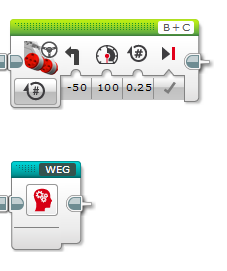
\includegraphics[width=5cm]{img/weg}
\label{fig:weg}
\end{figure}


\begin{table*}[]
\centering

\caption{Size in terms of the different number of blocks used in the seventeen \ms~programs, and the smells they exhibit}
\label{tab:robotica}
\sffamily
\begin{small}
\begin{tabular}{l|lllll|lll|lllllllll}
Name & L1  & L2 & L3  & L4  & L5  & L6  & L7  & L8  & L9  & L10 & L11 & L12 & L13 & L14 & L15 & L16 & L17 \\
\hline
Action       & 8  & 6  & 5  & 7  & 16 & 8  & 10 & 16 & 10 & 1  & 2 & 1  & 7  & 15 & 2 & 2  & 78  \\
Flow Control        & 3  & 5  & 4  & 4  & 4  & 3  & 7  & 11 & 2  & 2  & 1 & 4  & 11 & 2  & 0 & 0  & 25  \\
Sensor       & 1  & 0  & 0  & 2  & 1  & 0  & 8  & 10 & 4  & 1  & 0 & 1  & 0  & 4  & 2 & 0  & 0   \\
Data Operations      & 1  & 0  & 2  & 5  & 0  & 0  & 4  & 4  & 1  & 0  & 0 & 2  & 0  & 7  & 1 & 1  & 0   \\
Advanced & 0& 0 & 0 & 0 & 0 & 0 & 0 & 0 & 0 & 0 & 0 & 0 & 0 & 0 & 0 & 0 & 0 \\
MyBlock Call & 2  & 0  & 2  & 2  & 3  & 4  & 3  & 5  & 0  & 1  & 0 & 1  & 0  & 3  & 1 & 4  & 27  \\
\hline
Comment      & 2  & 0  & 0  & 1  & 0  & 0  & 1  & 0  & 0  & 6  & 6 & 0  & 15 & 0  & 0 & 7  & 13  \\
Variables    & 0  & 0  & 1  & 3  & 1  & 1  & 0  & 0  & 0  & 0  & 0 & 0  & 0  & 19 & 0 & 0  & 0   \\
MyBlocks     & 3  & 0  & 3  & 2  & 3  & 2  & 2  & 4  & 0  & 1  & 0 & 1  & 0  & 4  & 1 & 3  & 6   \\
\hline
Total Blocks        & 20 & 11 & 17 & 26 & 28 & 18 & 35 & 50 & 17 & 12 & 9 & 10 & 33 & 54 & 7 & 17 & 149\\
\hline
\hline
Dead Code                                              & \ding{51} &  & \ding{51} & \ding{51} &   &   & \ding{51} & \ding{51} &   &   &   &   &   & \ding{51} &   &   & \ding{51} \\
Deprecated                                          &   &  &   &   &   &   &   &   &   &   &   &   &   &   &   &   &   \\
Duplicate Code                                         &   &  &   & \ding{51} & \ding{51} & \ding{51} & \ding{51} & \ding{51} & \ding{51} & \ding{51} & \ding{51} &   & \ding{51} &   &   & \ding{51} & \ding{51} \\
Feature Envy                                           & \ding{51} &  & \ding{51} & \ding{51} &   &   &   &   &   &   &   &   &   &   &   &   &   \\
Inappropriate Intimacy                                 &   &  &   &   &   &   &   &   &   &   &   &   &   &   &   &   &   \\
Lazy Class                                             & \ding{51} &  & \ding{51} & \ding{51} &   & \ding{51} &   &   &   &   &   &   &   &   &   &   &   \\
Long method                                            &   &  &   &   & \ding{51} &   &   &   &   & \ding{51} &   &   &   & \ding{51} &   &   & \ding{51}   \\
Many Parameters                                        &   &  &   &   &   &   &   &   &   &   &   & \ding{51} &   &   &   &   &   \\
Message Chain                                          &   &  &   &   &   &   &   &   &   &   &   &   &   &   &   &   &   \\
No-op                                                  &   &  & \ding{51} &   &   &   &   &   &   &   &   &   &   & \ding{51} &   &   &  \\
Unused Field                                           &   &  &   & \ding{51} &   &   &   &   &   &   &   &   &   & \ding{51} &   &   &   \\
\hline
Total Smells & 3 & 0 & 4 & 5 & 2 & 2 & 2 & 2 & 1 & 2 & 1 & 1 & 1 & 4 & 0 & 1 & 3
\\
\end{tabular}
\end{small}
\end{table*}


\subsubsection{Study context}
To determine if EV3 programs suffer from OO-inspired smells, we  gathered 17 programs from two data sources. The first source is a robotics club run by one of the authors, where kids aged 8 to 13 program robots every week. Their programs have been collected as dataset for this paper. More specifically, we focus on two different projects within this set, RoboCup and Sumo. These two types of programs related to two different LEGO MINDSTORMS competitions: Sumo is a simple robot game in which robots have to `sumo wrestle' each other\footnote{\url{http://www.sugobot.com/}} and RoboCup Junior Rescue\footnote{\url{http://rcj.robocup.org/rescue.html}}, where robots have to navigate through a field and detect a soda can. Eight programs come from this source. 

To obtain a more diverse set of EV3 programs, we also solicited members of the EV3 programming group on Facebook to share their programs with us\footnote{\url{https://www.facebook.com/groups/legomindstorms/permalink/527560164058881/}}. Nine programs come from this second source. 

After collection, the programs were analyzed by one of the authors. Table \ref{tab:robotica} shows an overview of the EV3 programs, where programs L1 to L8 are programs from the robotics club (L1 to L5 are programs for Sumo and L6 to L8 are for RoboCup Junior) and programs L9 to L17  are programs received through Facebook. 

The EV3 programming interface divides the programming blocks into 6 categories, of which the number of blocks found in the programs is listed in the first 6 rows. Furthermore we have counted the number of comment blocks: special blocks that do not perform any action but are used to document programs, the number of variables: blocks that store a value that can be retreived later and the number of \mbs~ created in the program. The \emph{Total Blocks} column provides an indication of program size.  


\subsubsection{Findings}
When investigating the programs, we found that they indeed can suffer from OO-inspired smells. 

On average, the programs from children's robotics club had 2.5 smells each and the programs from the community received through Facebook had 1.4 smells each, though  the people submitting through Facebook most likely sent in nicely polished programs. Furthermore, the community programs were generally smaller (a median of 17 versus 23 total blocks) exhibiting more reuse as they more often used call to \mbs. There are only three smells that do not occur in any of the programs: \emph{deprecated interface} (not applicable), \emph{inappropriate intimacy} and \emph{message chain}.

Next, we discuss the three most common smells within the EV3 programs. 
%Duplicate Code occurs most, in over half of the programs. 

\begin{figure} [ht]
\caption{The project properties screen for the Sumo program 1, showing the three \mbs, but not indicating the \mb~`draaien' is currently not called anywhere.}
\centering
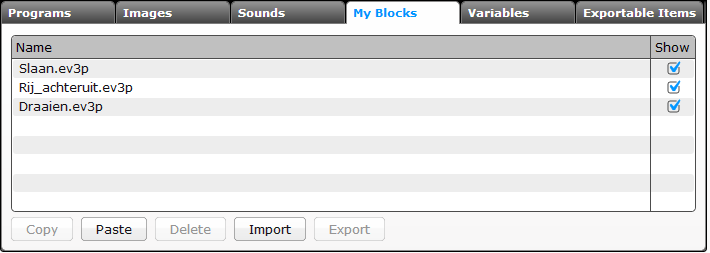
\includegraphics[width=\columnwidth]{img/overview-small}
\label{fig:overview}
\end{figure}

\paragraph{Duplicate Code}
The most common smell we found in the nine programs is the \emph{duplicate code} smell, which 11 out of 17 programs suffer from. Duplication comes in various forms.  Some of the programs use two motor blocks in a row, which could have been merged. For example, consider the two blocks from program L17, shown in Figure \ref{fig:dup_ev3}. This might have been challenging for the users to detect, as they use two slight variations of the motor block, but the two behave exactly the same in this case. Hence, one block moving forward 1.25 would have sufficed. Other programs exhibit duplication at a high level, such as the two \mbs~in program L16, depicted in Figure \ref{fig:dup_ev3_myblocks}. Here, the two \mbs~perform the exact same operation, but on a different motor. By connecting the name of the motor to a parameter two, this functionality could have been implemented with one \mb.

\begin{figure} [tb]
\caption{The duplication smell in two subsequent motor blocks. Since both have the same power and direction, they could have been merged. }
\centering
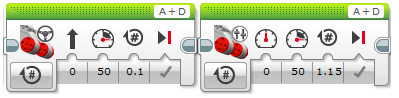
\includegraphics[width=\columnwidth]{img/dup_ev3}
\label{fig:dup_ev3}
\end{figure}

\begin{figure} [tb]
\caption{The duplication smell in two different \mbs. Both \mbs~turn a motor, and which motor could have been put in a parameter, like angle and speed already are. }
\centering
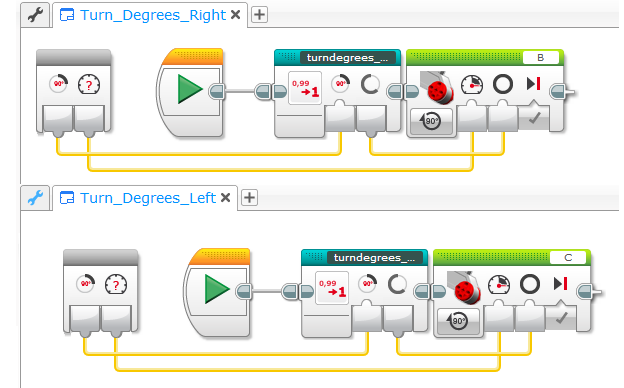
\includegraphics[width=\columnwidth]{img/dup_ev3_myblocks}
\label{fig:dup_ev3_myblocks}
\end{figure}

\paragraph{Dead Code}
The second most common smell is \emph{dead code}. In 7 out of 17 programs we found \mbs~that no longer connected to one of programs. This can pose a problem, as the EV3 environment compiles and transfers all programs and \mbs~to the physical brick, causing the memory to be full quite quickly. We see that \emph{dead code} is more common in the robotics class programs than in the programs we received via Facebook. This is probably due to the fact that these users felt confident enough to share their programs. Either the programs were reviewed before sharing them, or the experienced users selected `clean' programs to share.

Looking at the EV3 programming interface, it is not that surprising that users forget about disconnected \mbs. The interface does not help users in understanding what \mbs~are used. If we look at the project properties screen, shown in Figure \ref{fig:overview}, one can see that there is no information about which \mb~is used, and where. Even worse, users can delete \mbs~that are still being called, without a warning being issued about this. After removal of a \mb~ in use, the program no longer compiles.


\paragraph{Lazy Class}
A \emph{lazy class}, which we count as \mbs~containing three or fewer blocks, are also relatively common, occurring in four of the programs. However, we only find this smell in the programs from the robotics club and not in the programs received via Facebook. Many `lazy \mbs'~were relatively small, consisting of two or three blocks, or even one in some cases. In general, small abstraction are considered smelly, as understanding the abstraction requires inspecting it, which might not be worth it for small classes, methods or \mbs. However, the EV3 programming interface does not allow regular blocks to be named, but it does allow this for \mbs. So by making a \mb, users can express the intent of a coherent set of blocks, even if this set consist of just one block. 

As an example, consider the two blocks shown in Figure 5, where the left block is regular block controlling a motor, while the right one is a call to a \mb~with the same functionality. The first one just expresses what the robot must do, but the second one expresses the intent (`weg' meaning flee). By using the \mb, even with one block, the program gets easier to read.

\paragraph{Long method}
We defined Long Method as \mbs~with over 10 blocks, as this is typically the size that all blocks would not fit on the screen anymore. Long method occurs in four programs, but, contrary to Lazy Class, is found mostly in the Facebook programs. This is to be expected, as more experienced users can handle bigger \mbs, while the kids from the robotics club stick with making small blocks.

\subsubsection{Summary}
To summarize, smells indeed occur in the EV3 programs. Smells are found in 88\% of the programs, with \emph{duplicate code}, \emph{dead code} and \emph{lazy class} (small abstractions) observed most often. Hence we conclude that smells from OO are applicable to this end-user language, though programs might not be as smelly in the context of EV3 as they are in OO. 

\begin{figure}[ht]
\caption{The interface of Kodu~showing programming behavior for a bot.}
\centering
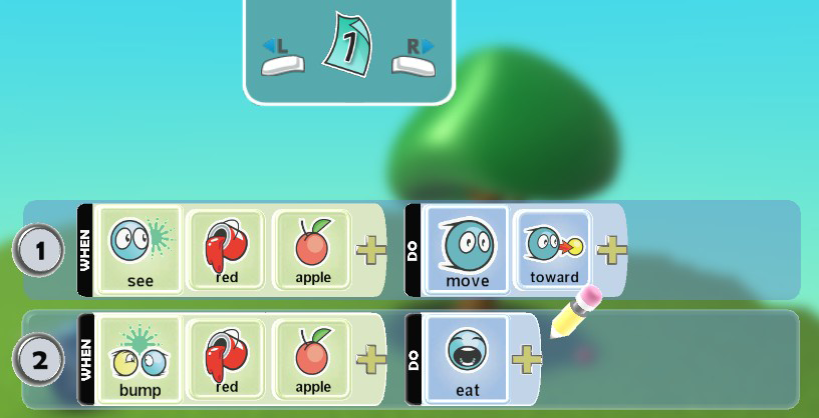
\includegraphics[width=\columnwidth]{programmingui.png}
\label{fig:Kodu}
\end{figure}


\subsection{Kodu}
Microsoft Research's Kodu is a visual programming language~\cite{kodugrammar} and environment that allows users to create, play, and share their own video games. 
It is available for download on the Xbox and PC and is heavily inspired by robotics, as illustrated by the context of programming in it and its language. 

Users create a world (e.g., land, water, clouds),  add characters and objects, and then can program each character or object (e.g., a kodu robot character, a turtle character, an apple object, a tree object; we use character and object interchangeably) individually. The programming defines how to interact with the world, treating each character or object as an autonomous agent. Each object has 12 pages that can be programmed, analogous to methods in an OO language, where the current page defines the current behavior of the object. 
The object's behavior can change by switching between pages to modify state and control flow. 
Each page contains a set of rules, and each rule is in the form of a condition and an action, which form a {\tt when~--~do} clause. The {\tt when} is defined by a sensor (e.g., see, hear, gamepad input) and filters (e.g., apple, gamepad A button). The {\tt do} is defined by an actuator (e.g., movement, shoot) and modifiers (e.g., missile, toward). All the rules on a page are evaluated in a single frame, from top to bottom. 
Despite its unique language, Kodu  can be used to express many basic concepts in computer science, such as variables, boolean logic and conditional control flow~\cite{Stolee:2011:ECS:1953163.1953197}. 

Figure~\ref{fig:Kodu} shows a page and two rules  in Kodu. For the first rule, the condition is, {\tt when see red apple}, and the action is, {\tt move toward it}. The action defines the behavior of this particular character when it sees a red apple, that is, it moves toward it. Since the condition identifies an object (i.e., apple), it becomes the default selector, even though it is not explicitly specified. The second rule has a similar condition with a different sensor, {\tt bump}. The action of the second rule, {\tt eat}, indicates that the character should eat any red apple it bumps. 
The programming in Figure~\ref{fig:Kodu} applies to the first page in this character's programming, as indicated by the number one at the top of the screen. The first page is the  start page.

To form more complex boolean logic, rules can also be indented to create complex {\tt when} clauses, where both conditions need to be true for the action to occur. Alternatively, indenting a rule and removing the {\tt when} means that multiple {\tt do} clauses occur for the same trigger condition. 





\subsubsection{Smells in Kodu}
We describe how the smells in our OO-inspired catalog apply to Kodu programs using a loose mapping of the OO concepts. We consider pages of programming as analogous to methods or classes, similar to how modules are treated in Yahoo Pipes, worksheets in spreadsheets and \mbs~in \ms. 

\begin{description}
\item[Dead Code:] If there exists a page with programming such that there is no explicit path of control flow from Page~1 to it, it is unreachable and therefore dead. 
\item[Deprecated Interface:] Some language features may exist in early versions of Kodu but not be available in future versions. As none of these features were ever deployed, this smell is not possible. 
\item[Duplicate Code:] Two pages for the same character with exactly the same set of rules, or two identical rules on a page constitute duplicate code. Alternatively, two rules on the same page with the same \emph{when} clauses (i.e., sensor and filter) but different actions could be consolidated using the indent feature and thus are smelly. 
\item[Feature envy:] All global variables, such as game scores, can be read and written by any character. If a certain character reads variables that have been written by another character, this could be an instance of the feature envy smell. 
\item[Inappropriate Intimacy:] A character has four local properties that describe its state: color, glow color, expressions (angry, crazy, happy). If one character frequently checks the properties of another character, this could constitute inappropriate intimacy. 
\item[Lazy Class:] If a character has no programming, it could be an instance of the lazy smell. 
%Characters with no programming are different than objects. Characters can have movement whereas objects cannot. 
\item[Long method:] A page with many, many rules may be difficult to understand. Some programming could potentially move to other characters. %We counted long methods as those with ten or more rules. 
\item[Many Parameters:] A game can have 37 different global scores. Games that use many of these could be unnecessarily smelly. %We set the threshold at three. 
\item[Message Chain:] It is possible for a character to create a chain of switches between pages without any logic on the page other than the jump. This would create a long and unnecessary message chain. 
\item[No-op:] Jumping to a page with no logic is the logical equivalent of a null pointer. While no error would be raised, the character would no longer have any behavior and would be stuck. Alternatively, rules with \emph{when} clauses but no \emph{do} clauses do not perform any actions. 
\item[Unused Field:] A global variable that is written to but not read is an instance of the the unused field smell. 

%\todo{emailed scoy at Microsoft about this}
\end{description}



\begin{table*}[]
\centering

\caption{Size in terms of the different number of characters and rules used in the 17 Kodu programs, and the smells they exhibit}
\label{tab:koduanalysis}
\sffamily
\begin{small}
\begin{tabular}{l | r@{\horiz }r@{\horiz }r@{ \horiz}r@{ \horiz}r@{\horiz }r@{ \horiz}r@{\horiz }r@{\horiz }r@{ \horiz}r@{ \horiz}r@{ \horiz}r@{\horiz }r@{\horiz }r@{ \horiz}r@{\horiz }r@{ \horiz}r@{\horiz } | r@{\horiz }r@{\horiz }r@{\horiz }r@{\horiz }r@{\horiz }r@{\horiz }r@{\horiz }r@{\horiz }r@{\horiz }r}
Name & K1  & K2 & K3  & K4  & K5  & K6  & K7  & K8  & K9  & K10 & K11 & K12 & K13 & K14 & K15 & K16 & K17 & K18 & K19 & K20 & K21 & K22 & K23 & K24 & K25 & K26 & K27\\
\hline
Characters        & 6&17&39&21&62&60&85&26&26&60&42&45&57&36&5&15&28
&28&10&2&16&18&76&75&63&4&76
\\
Pages 		&11&7&26&19&18&47&82&19&10&60&41&31&10&9&6&7&7
&34&16&2&39&18&9&50&90&8&78
\\
Rules 		&21&17&60&28&31&96&93&29&20&120&58&63&22&35&14&18&23
&114&54&3&113&27&30&122&144&32&372
\\
%Tiles        	& 90&64&252&150&121&418&535&141&66&227&230&244&81&159&54&90&103\\
HCI Actors & 1&2&1&1&2&1&1&1&1&1&1&1&1&0&2&1&1
& 5 & 1 & 0 & 0 & 1 & 1 & 1 & 37 & 0 & 2
\\
%\hline
%Total        & 20 & 11 & 17 & 26 & 28 & 18 & 35 & 50 & 17 & 12 & 9 & 10 & 33 & 54 & 7 & 17 & 149\\
\hline
\hline
Dead Code                                              &   &  &   &   &   &   &   &   &   &   &   &   &  \ding{51} &   &   &   &   
& & & & & & & \ding{51} & \ding{51} & &
\\
Deprecated                                          &   &  &   &   &   &   &   &   &   &   &   &   &   &   &   &   &   
& & & & & & &  & & & 
\\
Duplicate Code                                        &   &  & \ding{51}  &   &   & \ding{51}  & \ding{51}  & \ding{51}  & \ding{51}  &   &   & \ding{51}  &\ding{51}   & \ding{51}  &   & \ding{51}  &   
& \ding{51} & \ding{51} & \ding{51} & \ding{51} & \ding{51} & & \ding{51} & \ding{51} & & \ding{51}
\\
Feature Envy                                         &   &  & \ding{51}  &   &   &   &   &   &   & \ding{51}  &   &   &   &   &   &   &   
&  &  \ding{51}& & & & & \ding{51} & \ding{51} & & \ding{51}
\\
Inapprop. Int.                            &   &  &   &   &   &   &   &   &   &   &   &   &   &   &   &  \ding{51} &   
& & & & & & & & & &
\\
Lazy Class                                             &   & \ding{51} & \ding{51}  & \ding{51}  & \ding{51}  &\ding{51}   &\ding{51}   &\ding{51}   &\ding{51}   &   & \ding{51}  & \ding{51}  & \ding{51}  & \ding{51}  & \ding{51}  &  \ding{51} &\ding{51}   
& \ding{51} & & \ding{51} & \ding{51} & &  \ding{51}&  \ding{51}&  \ding{51}& & \ding{51}
\\
Long method                                        &  &  &  &   &   &\ding{51}   & &   & &   &   & \ding{51}  & \ding{51}  &   &   &   &    
&  \ding{51}& \ding{51} & & & & & \ding{51} & & & \ding{51}
\\
Many Params                                        &   &  &   &   &   &   &   &   &   &   &   &   &   &   &   &   &   
& & & & & & &  &  & & \ding{51}
\\
Message Chain                                          &   &  &   &   &   &   &   &   &   &   &   &   &   &   &   &   &   
& & & & & & & \ding{51} & & &
\\
No-op                                                  &   & \ding{51} &   &   &   &   &   &   &   & \ding{51}  &   & \ding{51}  & \ding{51}  & \ding{51}  &   &   &\ding{51}   
& & \ding{51} & \ding{51} & & & &  \ding{51}&  \ding{51}& & \ding{51}
\\
Unused Field                                           &   &  &  \ding{51} &   &   &   &   &   & \ding{51}  &   &   & \ding{51}  &   &   & \ding{51}  &   &   
&  \ding{51}& & & & & & & \ding{51} & & \ding{51}
\\
\hline
Total Smells & 0 & 2 & 4 & 1 & 1 & 3 & 2 & 2 & 3 & 2 & 1 & 5 & 5 & 3 & 2 & 3 & 2 
& 4&4 &3 &2 &1 &1 &7 &6 &0 &7
\\

\end{tabular}
\end{small}
\end{table*}


\subsubsection{Study Context}
To determine if Kodu programs indeed suffer from the above defined smells, we have gathered  programs from two data sources. 
For the first data source, we ran a workshop at the Microsoft FUSE lab that introduced children to Kodu Game Lab in a series of three 3-hour sessions.  To recruit participants, we advertised the Kodu workshop using a mailing list of parents interested in Kodu.  
Children between the ages of 9 and 12 volunteered to participate, with parental consent. We collected 17 programs created during the workshop for analysis. 
For the second data source, we randomly sampled 10 programs from the public Xbox Live community. No demographic information was collected about the users. 

The programs were analyzed  by one of the authors. Table~\ref{tab:koduanalysis} presents the 17 programs created by children (K1 \dots K17), 10 programs created by the Xbox Live community (K18 \dots K27), and the smells found in each. The \emph{Characters} row defines how many characters and actors are in the program, \emph{Pages} defines how many pages of programming are used by the characters, \emph{Rules} counts all the rules on all the pages, and \emph{HCI Actors} counts the number of actors in the program that are controllable by the Xbox controller, mouse, or keyboard. 
To count the number of instances of the \emph{long method}, a smell was counted when the page had 10 or more rules. For the  \emph{many parameters} smell, the use of four or more game scores. These thresholds were determined by the authors as 10 rules cannot be viewed on a screen screen without scrolling and only a couple games used more than three game scores. 

\subsubsection{Findings}
On average, the programs from children had 2.3 smells each and the programs from the community had 3.5 smells each, though we note that the programs from the community tend to be larger (e.g., an average of 101 rules vs. 42 rules). Next, we discuss the three most common smells found in the Kodu programs, appearing in 40\% or more of the sample. The remaining smells appear in 25\% or fewer programs. 

\subsubsection{Lazy class}
The lazy class smell was the most common, appearing in 79\% of the Kodu programs. This smell is intended to capture when a character is placed in the world but has no programming, and thus no behavior. In some cases, this may not be a smell at all, such as when characters are used as decorations in the world (e.g., trees and rocks). In others, it could be similar to an object that is created but that has no behavior. 

\subsubsection{Duplicate Code}
This smell was present in 61\% of the programs. All instances were that of duplicate {\tt when} clauses within a page, and there were no instances of identical rules on a page or identical pages within the same character. The prevalence of this feature shows a missed opportunity for consolidating the code. 

\subsubsection{No-op}
The next most-common smell is the no-op, present in 41\% of the programs. All instances of this smell were rules without {\tt do} clauses, rather than jumping to pages without logic.  This is probably the product of the rapid cycling between testing and developing observed in Kodu development~\cite{Stolee:2011:ECS:1953163.1953197}; since the clauses have no actionable logic, keeping them in the code does not impact the semantics of the program. We note that none of the rules following these clauses were indented to create a conditional conjunction. 


\subsubsection{Summary}
To summarize, smells indeed occur in the Kodu programs. Smells are found in 93\% of the programs, with \emph{lazy class}, \emph{duplicate code},  and \emph{no-op} (small abstractions) appearing most often. Hence we conclude that smells from OO are applicable to this end-user language. 

\subsection{Summary}
Table~\ref{tab:smellsummary} summarizes the frequencies of occurrence of the various smells in the EV3 and Kodu programs. Overall, 88\% of the EV3 and 93\% of the Kodu programs contained at least one smell. Coupled with the 81\% of Yahoo Pipes programs~\cite{StoleeTSE2013} and 42\% of Excel programs~\cite{Hermans2012intra} that were previously found to be smelly, this provides further evidence of the prevalence of smells in end-user programs. 

As with code written by other end-user programmers~\cite{StoleeTSE2013}, \emph{duplicate code} is prevalent in EV3 and Kodu programs, affecting over 60\% of the samples in both languages. The other two smells that were studied in Excel and Yahoo Pipes, \emph{lazy class} and \emph{long method}, are present in at least 24\% of the studied EV3 and Kodu programs, illustrating commonality across all end-user programming domains. 

\emph{Dead code} is more frequently found in EV3 and \emph{lazy class} smells are more common in Kodu. The \emph{no-op} smell is present in 41\% of the Kodu programs, which is similar in spirit to the 41\% of EV3 programs with \emph{dead code}. \emph{Feature envy} was also prevalent across both languages, appearing in 18\% and 22\% of the EV3 and Kodu programs, respectively. 
We observe that the occurring smells seem to be anti-patterns that occur in programming in general, independent of the programming language. 

\begin{table}
\caption{Summary of Smells Across EV3 and Kodu Programs \label{tab:smellsummary}}
\begin{small}
\begin{center}
\begin{tabular}{l | r r}
&EV3&Kodu\\ \hline
Dead Code&41\%&11\%\\
Deprecated Interfaces & 0\% & 0\%\\
Duplicate Code&65\%&61\%\\
Feature Envy&18\%&22\%\\
Inappropriate Intimacy&0\%&4\%\\
Lazy Class&24\%&79\%\\
Long method&24\%&25\%\\
Many Parameters&6\%&4\%\\
Message Chain&0\%&4\%\\
No-op&12\%&41\%\\
Unused Field&12\%&25\%\\ \hline
Any smell & 88\% & 93\%
\end{tabular}
\end{center}
\end{small}
\end{table}

\section{Beyond OO Smells}
\label{sec:beyond}

\label{sec:smells:domain}
The end-user programming environments offer many opportunities to define smells based on user behavior or unique elements of the domain. Here, we explore opportunities for new smells in end-user domains that extend beyond the OO-inspired smells in Section~\ref{sec:smells}. 

\subsection{End-User Programming Smells}
Many smells beyond the OO language exist in several of the domains studied. 

\subsubsection{Layout smells}
The EV3 and Yahoo Pipes languages are visual and involve connecting boxes with wires, making it easy to create an unwieldily structure. EV3 is especially problematic as it lacks an auto-layouting function.

A special case where this happens is when a user creates a \mb. Remember that \mbs~can only be created with an `extract method' operation. If this operation is called, all selected are moved to the newly created \mb, and are replaced by one block that is a call to this new \mb. Other than that, the layout remains unchanged. So if a big \mb~is created, the program will now have a big gap, making the program harder to read \todo{if room show example}. This, and other layout smells too are unique to visual languages and can impede understandability. 

%Katie just realized this is true of ALL LANGUAGES EVERYWHERE, since most don't fit on whatever screen. Oops. 
%\subsubsection{Lack of Visual Abstraction smell}
%Visual languages can suffer from a visual lack of abstraction smell when the entire program does not fit well on the screen and thus is difficult to comprehend. The threshold for the presence of this smell is clearly dependent on screen size, but nonetheless, it can have an impact on program maintainability~\cite{StoleeTSE2013}. 
%
%This is similar to the \emph{long method} smell in Kodu and EV3, the \emph{duplicate code} smell in Yahoo Pipes (named \emph{isomorphic paths}), or \emph{many operations} in Excel.
%	
%One way to deal with this kind of visual smell is through abstraction. The Yahoo Pipes language provides this through the subpipe module, EV3 through MyBlocks, and Excel through worksheets.  Including subpages or being able to collapse rules on a page would facilitate this in Kodu but support for that is currently not available. 


\subsubsection{Lack of Comments smell}
The lack of comments in a program can make it difficult to understand. Kodu and Yahoo Pipes both suffer form a lack of comments in the programming language and development environment, often making it difficult to understand another's work or maintain old code. 


\subsubsection{Programming Organization smell}
Communities of programmers often have standards for how to structure program code. These \emph{population-based} smells were first introduced for Yahoo Pipes~\cite{StoleeTSE2013} and can be uncovered by exploring programs written by the community. In Kodu, often the rules that map a character's behavior to user input from a gamepad, keyboard or mouse are at the top of a page and the remaining logic is at the bottom. Deviating from this structure can lead to programs that are more difficult to understand when shared. 

\subsection{Domain-Specific Smells}
Each end-user domain has unique characteristics that create opportunities for defining domain-specific smells. In Yahoo Pipes, prior work has explored the presence of broken or deprecated data sources as a smell unique to the domain~\cite{StoleeTSE2013}. In Excel, prior work defined referring to an empty cells are smelly~\cite{cunha2012towards}. Here, we explore smells in EV3 and Kodu that are unique to their languages and environments. 

\subsubsection{EV3}
%\subsubsection{Hardware/Software Interface Smells}
The \ms~programming language differs significantly from the other end-user domains, as EV3 programmers work with both software and hardware. While programming, users need to configure motor blocks to the right port, for example the blocks in Figure \ref{fig:dup_ev3} are controlling motors A and D. This means that, when a user has the wrong mental model of what motor is connected to what port, the program will not function as wanted. It appears users run into this issue too, as some of the programs we saw comment blocks where the mapping was described, in an effort to ensure proper mapping \todo{if room add example}.

Hence a smell unique to the EV3 domain is a wrong mapping between the robot in reality and the motor and sensor blocks. 

%Not sure if we should add this, but I have the rule in class that you can only raise your hand to ask a question if you have checked the mapping. And it still goes wrong often. 

\subsubsection{Kodu}
The Kodu environment involves designing games, programming games, and playing games. This, paired with the unique event-driven language, creates unique opportunities for domain-specific Kodu smells. 

% 


\paragraph{Conflicting Outcomes smell}
The event-driven language in Kodu allows a user to write conflicting outcomes for the same trigger, that is, with the same \texttt{when} clause, to write conflicting \texttt{do} clauses. For example, consider the following two Kodu rules:
\begin{verbatim}
(1) When hear turtle : do score 1 red
(2) When hear turtle : do unscore 1 red
\end{verbatim}
\noindent The \emph{do} clauses are in conflict, both scoring and unscoring the red score by 1, and hence the outcome is the same. Flagging conflicting rules during development would help alert users to this smell. 

\paragraph{Single Input Device smell}
Games in Kodu can be programmed and played using an Xbox controller or a keyboard and mouse. Many games are programed assuming a particular device for input, such as an Xbox. However, when playing a game in a different environment, that device may not be available, and thus the game is not portable. This smell could be mitigated by adding analogous rules for other input devices, such as mapping the gamepad trigger switches to the keyboard shift keys or mapping the right stick to movement. 

\paragraph{Lost Character smell}
The \emph{lazy class} smell is related to a non-programmed character or object. However, there is also a design smell that can manifest when a programmed object cannot be easily found in the world, and thus there is program behavior that is difficult to change. Resolving this smell could involve physically moving the characters or objects to be more accessible, adding a color or speech bubble above them as a marker, or by adding an environment feature that maintains a list of programmed and non-programmed characters that can be accessed. 	

\section{Related Work}

\label{sec:related_work}
Related to the current research are efforts on code smells within traditional languages, starting with the work of Fowler\cite{Fowl1999}. His book gives an overview of code smells and corresponding refactorings. Recent efforts focused on the automatic identification of code smells by means of metrics. Marinescu~\cite{Mari2001} for instance, uses metrics to identify \emph{suspect} classes, those classes that might have design flaws. Lanza and Marinescu~\cite{Lanz06} explain this methodology in more detail. Alves \emph{et al.}~\cite{Alves2010} focus on a strategy to obtain thresholds for metrics from a benchmark. Olbrich \emph{et al.} furthermore investigates the changes in smells over time, and discusses their impact~\cite{Olbr2009}.

Within end-user programming, this paper builds upon two lines of related work. First, the work of Stolee and Elbaum that studied smells~\cite{StoleeTSE2013} and refactorings~\cite{Stolee2011}. They designed a number of smells by transforming known OO smells to the domain of Yahoo Pipes. The second direction is the work by Hermans \emph{et al.} that also took OO smells as an inspiration from a number of smells~\cite{Hermans2012intra, Hermans2012inter}. Subsequently they described corresponding refactorings~\cite{Hermans2012intraExt} and a tool that applies refactorings~\cite{hermans2014bumblebee}. This final work builds upon previous work by Badame and Dig that described the first spreadsheet refactoring tool RefBook~\cite{badame2012refactoring}.

In end-user programming environments, user input and logic are often more closely linked than they are in general purpose languages, and as such analyzing the input data as opposed to the logic can also be used as a means of \emph{smell detection}. This is a direction that has been applied to spreadsheets. Cunha et. al \cite{cunha2012towards} for example look at anomalies in the data and define these as smells. Examples of this are \textit{Standard Deviation} which occurs if one assumes a normal distribution for a column in numeric values and the column contains values which fall outside two standard deviations. In more recent work, Barowy et. Al \cite{barowy2014checkcell} take a more formalized approach which they label ``Data Debugging''. Their solution uses statistical analysis to find values with an unusually high impact on the calculated results in a spreadsheet, as such values are likely either very important or erroneous.

In addition two above described work on Yahoo Pipes and spreadsheets, there is previous smells work on other end-user environments too, like performance smells in LabView, a visual language for system-design~\cite{chambers2013smell, chambers2015impact}. 

Research related to  EV3 and Kodu predominantly explores 
language design~\cite{Fristoe:2011:SSE:2159365.2159396, Stolee:2011:ECS:1953163.1953197, MacLaurin:2009:KEP:1536513.1536516, MacLaurin:2011:DKT:1925844.1926413} 
and educational benefits~\cite{Fowler:2011:KGL:2159365.2159398, Touretzky:2013:AKC:2445196.2445374, Barnes:2002:TIJ:563340.563397, Hood:2005:TPL:1067445.1067454}. 
%The language of Kodu can be used to express computer science concepts commonly taught in introductory classes, such as boolean logic, variables, and objects~\cite{Stolee:2011:ECS:1953163.1953197}. 
There is some, albeit limited, work on detecting code smells in educational languages. Chatley and Timbul describe Kenya, a simple programming language for educational purposes, which they have integrated into the Eclipse environment~\cite{Chatley2005}. They built features that allow the detection of `bad style' in programs to be detected and reported as code is written, concentrating on encouraging students to program like they were taught in class. This work might indicate that smell detection can be useful for education, but the authors  did notevaluate the usefulness of this approach.


%\section{Discussion}
%\label{sec:discussion}
%
%Based on the research and results for smell detection in end-user programming domains, there are many directions for future work in the domains studied and other end-user domains.
%
%



\section{Threats to Validity}
\label{sec:threats}
The threats to validity of this work inherit the threats to validity of the original studies~\cite{Stolee2015, Stolee2011, StoleeTSE2013, Hermans2011, Hermans2012intra, Hermans2012inter, hermans2014bumblebee, badame2012refactoring} on end-user refactoring in spreadsheets and Yahoo Pipes.

%Furthermore, research in smells and spreadsheets has focused on Microsoft Excel. However, other spreadsheet software exists and operates on the same principles. Thus there is also an opportunity to confirm that the identified smells apply in other spreadsheet software.

Three domains studied in this paper all happen to be dataflow languages, and the smells and refactorings may not generalize to other end-user programming domains (e.g., Scratch is OO-based). However, we mitigate this threat by analyzing Kodu, an event-driven language, and show that the 
smells are also applicable in that context. This provides more evidence of the generality of these smells. 
%\todo{katie, would you say Kodu is dataflow based too?} \todo{no, Kodu is an event-driven language}

We have defined OO smells in two languages, EV3~and Kodu, yet we have not evaluated whether these smells matter to the end users. Future work is needed to determine the impact of these smell on users of the languages. 

In Kodu, the presence of the \emph{lazy class} smell may be intentional and simply represent a design decision (i.e., a rock is not programmed because it's there purely for aesthetics). Evaluating these smells with actual users will help tease out when code is smelly and when it is actually designed intentionally. 

We have sampled programs from two sources for each EV3 and Kodu, yet these programs may not be representative of what children and community members create. A larger-scale analysis is necessary to generalize these findings to the populations of EV3 and Kodu programs. 

\section{Conclusion}
\label{sec:conclusions}
This paper presents an overview of the work in smell detection for end-user programming languages. More specifically, it synthesizes work on Yahoo Pipes and Excel into a catalog of generally applicable smells in end-user languages. To demonstrate the applicability of the catalog, we apply it to two new domains: \ms~and Kodu, two visual languages aimed at programming education. The results show that indeed many of the catalog's smells apply in the new domains, and \emph{lazy class} (small abstractions), \emph{duplicate code} and \emph{dead code} occur frequently in these educational languages too, while being of a quite different character than the textual languages aimed at professional developers that the smells were originally defined for. This shows the applicability of these smells, and also warrants further research into issues end-users encounter while programming. The contributions of this paper are:

\begin{itemize}
	\item A catalog of object-oriented-inspired code smells in end-user programs (Section \ref{sec:smells})
	\item Application of the catalog to two new end-user domains focused on education (Section \ref{sec:application})
	\item Identification of future opportunities for smell detection in end-user programming domains, both within and beyond the OO paradigm (Section \ref{sec:beyond})
\end{itemize}

The current work also gives rise to more research, for example, exploring the impact of code smells on children who use the educational languages or designing user-friendly refactoring tools for visual languages. 

%sentence from the original intro, I think I like it better here, it feels reflecting
In the end, we observe that the applicability of smells, originally created to detect weaknesses in source code, to other domains shows how powerful the concept is. Furthermore, studying the smells in a fresh context provides new insight on how to use smells in software engineering \todo{do we show this insight on how to use smells in SE?} and even suggests new types of smells. 

\balance

\section*{Acknowledgements}
Special thanks to Stephen Coy for his help with Kodu. This work is supported in part by  NSF SHF-EAGER-1446932 and the Harpole-Pentair endowment at Iowa State University.
\todo{Felienne - do you have funding to support or people to thank, like the community center?}

\bibliographystyle{IEEEtran}
\bibliography{literaturelist}

\end{document}

